\chapter{TraMoS in the TESS era}\label{chap:tess}

With the end of the Kepler mission, thousands of possible exoplanets remain as candidates known as Kepler Objects of Interest (KOI). The Kepler Object of Interest Network (KOINet: \citep{vonEssen2018,Freuddenthal2018}) in the Northern hemisphere, is a network of ground-based telescopes performing photometric follow-up of KOIs to continue what Kepler left undone. The main goal of KOINet is to combine Kepler data with ground-based observations in order to confirm and characterise the masses of exoplanet candidates using TTVs.

It is crucial for TTV studies to continue the work of space missions from ground. It is unlike to only with space-based observations to cover the interaction timescales to dynamically prove the TTV signal and the existence of some exoplanets companions, as in shown in Figure \ref{koinet} from the KOINet project. In this figure, new data from ground-based telescopes were fundamental to confirm the TTV signal, and therefore to perform a proper characterization of the system.

\begin{figure}
\centering
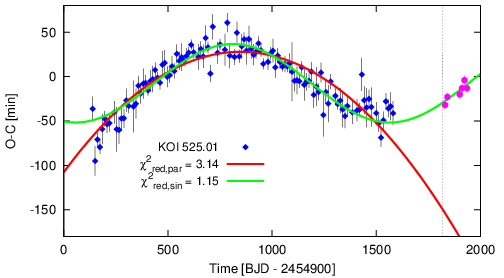
\includegraphics[width=0.7\columnwidth]{imagenes/koinet.png}
\caption{Observed minus calculated (O-C) diagram of the KOI-525b transit times, from the KOINet project. The observations from Kepler are in blue, and two different models were fitted on those data: an orbital decay model is in red, and a periodical TTV model is in green. If only Kepler data is considered, the two model could be plausible. The new ground-based observations (in pink) were essential to confirm the TTV nature of the system, discarding an orbital decay}
\label{koinet}
\end{figure}

The new space telescope Transiting Exoplanet Survey Satellite (TESS: \cite{Ricker2014}) is providing its first discoveries. The TESS observation plan divided in 13 sectors will challenge the confirmation process and characterization of possible exoplanets. During the $\sim27$ days of each sector, many candidates will not be observed enough time to confirm and characterize them. However, this special feature will provide a huge amount of new transit events of already known transiting exoplanets. Combining the new TESS data with ground-base follow- up observations, many possible TTVs could be confirm or rule out. Moreover, \cite{Ballard2018} predicted that around 5\% of the planets discovered by TESS will exhibit measurable TTV signals, similar to Kepler’s results.

Thus, for the future stage of the TraMoS project, archival data - collected since 2008 - will be combined with the upcoming TESS data and new ground-based observations using one-meter class telescopes. 


